\subsection{Team- und Partiekonfigurator}
Diese Komponente enthält einen Konfigurator, mit dem sich sowohl Quidditch-Teams, als auch Partien konfigurieren lassen.

\subsubsection{Schnittstellenarten}
Als Benutzerschnittstelle wird, wie im Lastenheft vorgeschrieben, eine GUI verwendet. \textbf{Begründung:} Der Nutzer möchte alle Informationen zu einer gegebenen Konfiguration übersichtlich dargestellt bekommen und anhand dieser Darstellung direkt Änderungen vornehmen können. Hierfür ist eine GUI die intuitivste und sinnvollste Variante, da eine grafische Darstellung eine übersichtliche Visualisierung erlaubt und eine Änderung direkt anhand dieser Visualisierung möglich ist. Zudem könnte auf diese Weise die Komponente reibungslos in die Client-Anwendung integriert werden, falls man zu einem späteren Zeitpunkt den Konfigurator im Menü der Client-Anwendung direkt aufrufen möchte.

\subsubsection{Dialoge}
Im Folgenden werden den bereits formulierten Anforderungen und Anwendungsfällen der Komponente den entsprechenden Dialogen zugeordnet.

\begin{figure}[H]
    \centering
    \begin{tabular}{| l l l l |}
    \hline
    \textbf{Name} & \textbf{Typ} & \multicolumn{2}{l|}{\textbf{Abgedeckte Anwendungsfälle}} \\\hline
    Konfiguratormenü & Dialog & QA18 & implizit aus Benutzerfreundlichkeit\\\hline
    Teammenü & Dialog & QA18 & implizit aus Benutzerfreundlichkeit\\\hline
    Team laden & Dialog & FA72 & Konfiguration öffnen \\\hline
    Teamkonfigurator & Dialog & FA70-72 & Konfiguration erstellen/bearbeiten\\\hline
    Team speichern & Dialog & FA72 & Konfiguration speichern \\\hline
    Partiemenü & Dialog & – & implizit, da Strukturierung erforderlich\\\hline
    Partiekonfiguration laden & Dialog & FA72 & Konfiguration öffnen \\\hline
    Partiekonfigurator & Dialog & FA70-72 & Konfiguration erstellen/bearbeiten\\\hline
    Partiefonfiguration speichern & Dialog & FA72 & Konfiguration speichern \\\hline
    Konfiguration erfolgreich & Popup & QA17-18 & Benutzerfreundlichkeit und Robustheit\\\hline
    Konfiguration ungültig & Popup & QA17-18 & Benutzerfreundlichkeit und Robustheit\\\hline
    \end{tabular}
\end{figure}

\subsubsection{Dialogstrukturdiagramme}    
\begin{figure}[H]
    \centering
    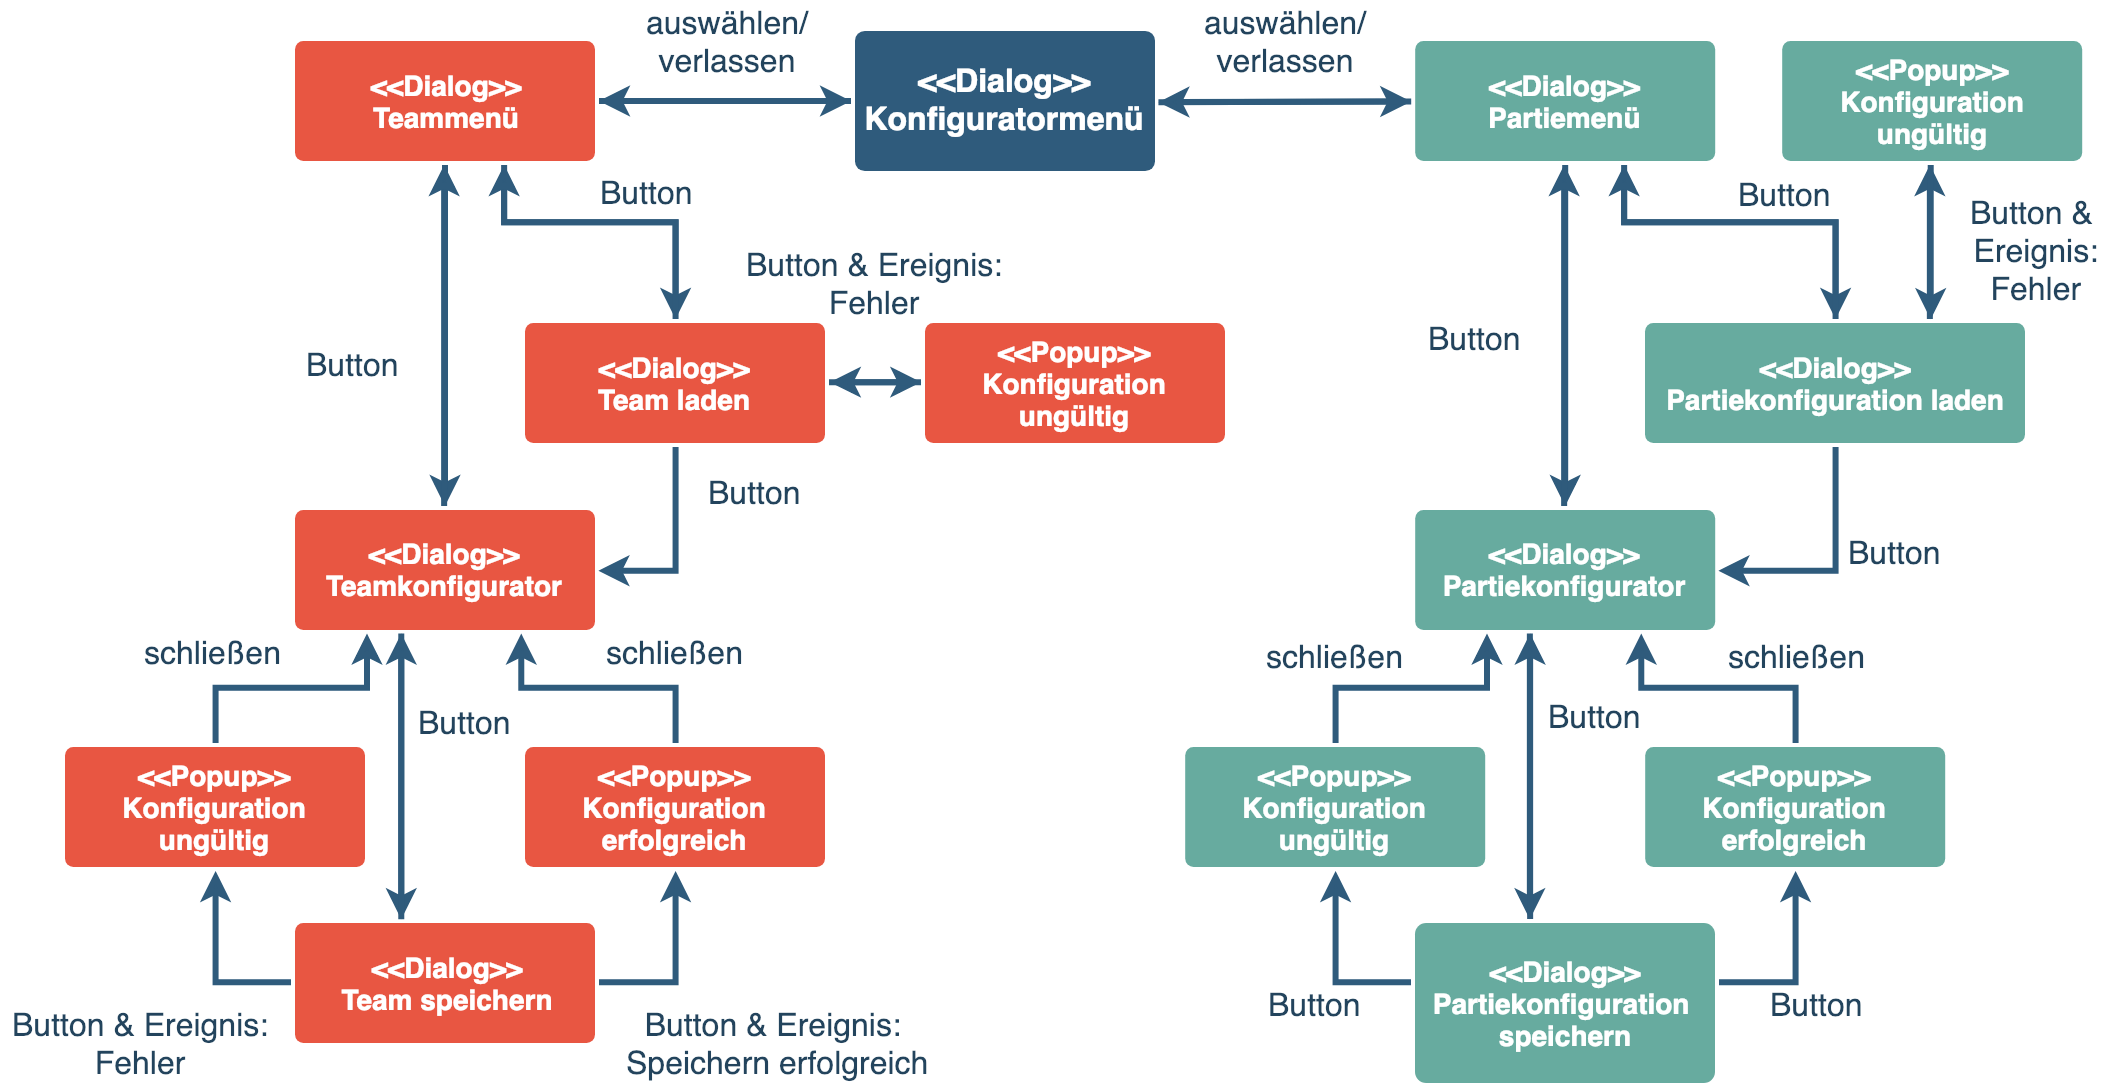
\includegraphics[width=\textwidth]{images/dialogstruktur_konfigurator}
\end{figure}



